\begin{enumerate}[label=\textbf{\arabic*.}, leftmargin=1.8em, itemsep=9pt, topsep=0pt, start=10]
    \item Nếu $f$ khả vi tại $a$, với $a > 0$, hãy tính giới hạn sau theo $f'(a)$:
    \[
    \lim_{x \to a} \frac{f(x) - f(a)}{\sqrt{x} - \sqrt{a}}
    \]

    \item Hình vẽ cho thấy một đường tròn bán kính 1 nội tiếp trong parabol $y = x^2$. Tìm tâm của đường tròn.
    \begin{center}
        \vspace{1pt}
        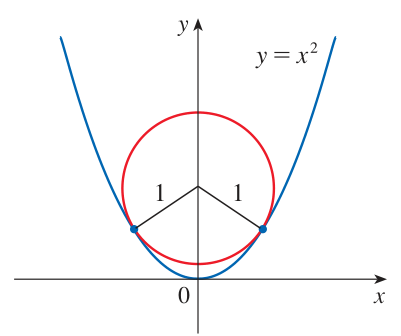
\includegraphics[width=0.44\linewidth]{images/p0311_fig1.png}
        \vspace{-2pt}
    \end{center}

    \item Tìm tất cả các giá trị của $c$ sao cho các parabol $y = 4x^2$ và $x = c + 2y^2$ cắt nhau vuông góc.

    \item Có bao nhiêu đường thẳng tiếp xúc với cả hai đường tròn $x^2 + y^2 = 4$ và $x^2 + (y - 3)^2 = 1$? Các tiếp tuyến này tiếp xúc với các đường tròn tại những điểm nào?

    \item Nếu $f(x) = \dfrac{x^{46} + x^{45} + 2}{1 + x}$, hãy tính $f^{(46)}(3)$. Biểu diễn câu trả lời của bạn bằng ký hiệu giai thừa:
    \[
    n! = 1 \cdot 2 \cdot 3 \cdots (n - 1) \cdot n
    \]

    \item Hình vẽ cho thấy một bánh xe đang quay có bán kính $40\text{ cm}$ và một thanh truyền $AP$ có chiều dài $1{,}2\text{ m}$. Chốt $P$ trượt qua lại dọc theo trục $x$ khi bánh xe quay ngược chiều kim đồng hồ với tốc độ 360 vòng/phút.
    \begin{enumerate}[label=\textbf{(\alph*)}, leftmargin=*, itemsep=1.5pt, topsep=2pt]
        \item Tìm vận tốc góc của thanh truyền, $d\alpha/dt$, theo radian trên giây, khi $\theta = \pi/3$.
        \item Biểu diễn khoảng cách $x = |OP|$ theo $\theta$.
        \item Tìm một biểu thức cho vận tốc của chốt $P$ theo $\theta$.
    \end{enumerate}
    \begin{center}
        \vspace{2pt}
        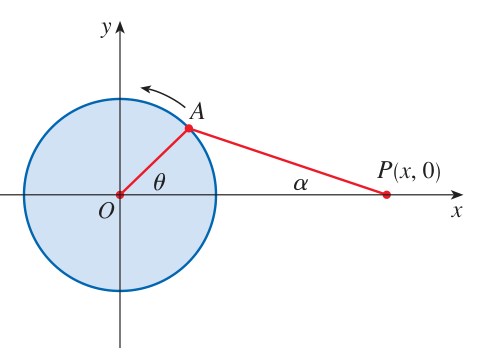
\includegraphics[width=0.54\linewidth]{images/p0311_fig2.png}
        \vspace{-2pt}
    \end{center}

    \item Các tiếp tuyến $T_1$ và $T_2$ được kẻ tại hai điểm $P_1$ và $P_2$ trên parabol $y = x^2$ và chúng cắt nhau tại điểm $P$. Một tiếp tuyến khác $T$ được kẻ tại một điểm nằm giữa $P_1$ và $P_2$; nó cắt $T_1$ tại $Q_1$ và cắt $T_2$ tại $Q_2$. Chứng minh rằng
    \[
    \frac{|PQ_1|}{|PP_1|} + \frac{|PQ_2|}{|PP_2|} = 1
    \]

    \item Chứng minh rằng
    \[
    \frac{d^n}{dx^n}(e^{ax} \sin bx) = r^n e^{ax} \sin(bx + n\theta)
    \]
    trong đó $a$ và $b$ là các số dương, $r^2 = a^2 + b^2$, và $\theta = \tan^{-1}(b/a)$.
\end{enumerate}

\par\vspace{3pt}%
\noindent\llap{\makebox[2.5in][l]{\hspace{0.4in}\textbf{\textsf{\Large 276}}}}%
